\documentclass{ximera}

\input{../preamble.tex}

\author{Gregory Hartman \and Matthew Carr}
\license{Creative Commons 3.0 By-NC}
\acknowledgement{https://github.com/APEXCalculus}

\begin{document}
\begin{exercise}

\tag{derivative}


\outcome{Understand the derivative as a function related to the original function.}
\outcome{Use the first derivative to determine whether a function is increasing or de- creasing.}


Using the graph of $g(x)$ shown below, answer the following questions. Write unions/intersections of intervals going from left to right on the number line.

\noindent\begin{minipage}[t]{.49\linewidth}
\begin{enumerate}
\item		Where is $g(x) > 0$?
\item		Where is $g(x) < 0$?
\item		Where is $g(x) = 0$?
\end{enumerate}
\end{minipage}
\begin{minipage}[t]{.49\linewidth}
\begin{enumerate}\addtocounter{enumi}{3}
\item		Where is $g'(x) < 0$?
\item		Where is $g'(x) > 0$?
\item		Where is $g'(x) = 0$?
\end{enumerate}
\end{minipage}

\begin{center}
\noindent\begin{minipage}[t]{.5\linewidth}
 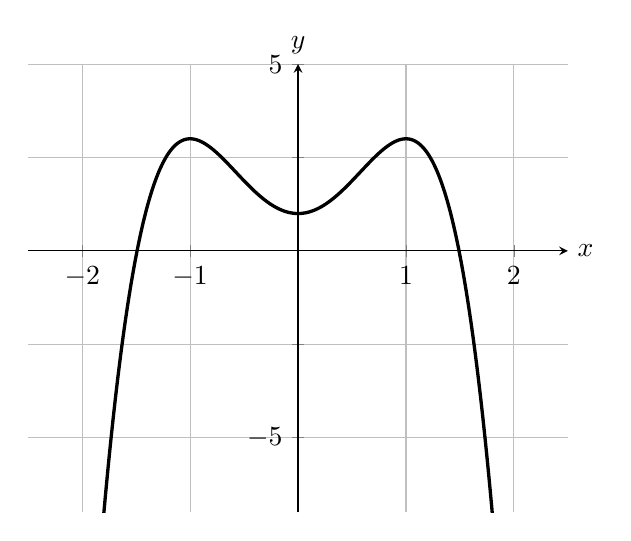
\begin{tikzpicture}
	\begin{axis}
	[ymin=-7,ymax=5, xmin=-2.5,xmax=2.5, axis lines=center,xlabel=$x$,ylabel=$y$,every axis y 
	label/.style={at=(current axis.above origin),anchor=south},every axis x label/.style={at=(current axis.right of origin),anchor=west},
	domain=-3:3,
	ytick={-5,-2.5,0,2.5,5},
	yticklabels={$-5$,,,,$5$},
	xtick={-2,-1,1,2},
	xticklabels={$-2$,$-1$,$1$,$2$},
	ymajorgrids=true,
	grid = major
	]
	\addplot[domain=-2:2,very thick,smooth,samples=1000]
	{4*pow(\x,2)-2*pow(\x,4)+1};
	\end{axis}
       \end{tikzpicture}
\end{minipage}
\end{center}


\noindent\begin{minipage}[t]{.49\linewidth}
\begin{enumerate}
\item		On $\begin{prompt}(\answer{-1.5},\answer{1.5})\end{prompt}$
\item		On $\begin{prompt}(\answer{-\infty},\answer{-1.5}) \cup (\answer{1.5},\answer{\infty})\end{prompt}$
\item		At $x\begin{prompt} = \pm\answer{1.5}\end{prompt}$
\end{enumerate}
\end{minipage}
\begin{minipage}[t]{.49\linewidth}
\begin{enumerate}\addtocounter{enumi}{3}
\item		On $\begin{prompt}(\answer{-\infty},\answer{-1})\cup(\answer{0},\answer{1})\end{prompt}$
\item		On $\begin{prompt}(\answer{-1},\answer{0})\cup(\answer{1},\answer{\infty})\end{prompt}$
\item		At $x\begin{prompt} = \pm\answer{1}\end{prompt}$
\end{enumerate}
\end{minipage}

\end{exercise}
\end{document}
